\documentclass[11pt,a4paper,twocolumn]{article}
\usepackage[utf8]{inputenc}
\usepackage[T1]{fontenc}
\usepackage{lmodern}
\usepackage{amsmath,amssymb,amsfonts}
\usepackage{graphicx}
\usepackage{xcolor}
\usepackage{titlesec}
\usepackage{tikz}
\usepackage{pgfplots}
\usepackage{geometry}
\usepackage{hyperref}
\usepackage{multicol}
\usepackage{booktabs}
\usepackage{float}
\usepackage{lipsum}

\geometry{left=1.5cm,right=1.5cm,top=2cm,bottom=2cm}
\usetikzlibrary{shapes.geometric, arrows, positioning, fit, calc}
\pgfplotsset{compat=1.18}

% Custom Colors
\definecolor{primary}{RGB}{0, 71, 143}
\definecolor{accent}{RGB}{200, 30, 30}
\definecolor{lightgray}{RGB}{240, 240, 240}
\definecolor{border}{RGB}{100, 100, 100}

% Title Formatting
\titleformat{\section}{\large\bfseries\color{primary}}{\thesection}{1em}{}[\titlerule]
\titleformat{\subsection}{\normalsize\bfseries}{\thesubsection}{1em}{}

% Diagram Styles
\tikzstyle{device} = [rectangle, rounded corners, minimum width=2.5cm, minimum height=1cm, text centered, draw=border, fill=white, font=\bfseries\small]
\tikzstyle{fpga} = [rectangle, minimum width=3cm, minimum height=1cm, text centered, draw=primary, fill=primary!10, font=\bfseries\small]
\tikzstyle{arrow} = [thick,->,>=stealth, color=border]
\tikzstyle{block} = [rectangle, draw=border, fill=white, text width=2cm, text centered, rounded corners, minimum height=1.2cm, font=\small]
\tikzstyle{pool} = [rectangle, draw=accent, fill=accent!10, text width=2cm, text centered, rounded corners, minimum height=1.2cm, font=\small]

\title{\vspace{-1.5cm}\Huge\bfseries\color{primary} Pareto 03 Architecture \\ \Large ECG Harware Accelerator on Virtex-6 ML605}
\author{\large System-on-Chip \& Hardware Acceleration Lab}
\date{\vspace{-0.5cm}\today}

\begin{document}

\maketitle
\thispagestyle{empty}

\begin{abstract}
This document details the architecture, design methodologies, and physical implementation constraints for the \textbf{Pareto 03} Convolutional Neural Network (CNN) specifically tailored as a hardware accelerator for 4-class Arrhythmia classification. Transitioning from traditional hand-coded Verilog to an H100 Genetic Algorithm-optimized \textit{Pareto front}, this iteration delivers state-of-the-art inference efficiency within the constraints of a Xilinx Virtex-6 ML605 FPGA.
\end{abstract}

\section{Introduction \& Methodology}

The transition from a manual RTL design (baseline \texttt{Multi} module) to an automated Neural Architecture Search (NAS) represents a paradigm shift from ``Hardware-First'' to ``ML-Hardware Co-Design''. Using an H100 GPU cluster, the NSGA-II (Non-dominated Sorting Genetic Algorithm II) generated thousands of potential network topologies. Rather than maximizing accuracy exclusively, NSGA-II simultaneously rewarded networks that minimized DSP, BRAM, and parameter footprint.

The chosen candidate, \textbf{Pareto 03}, resides directly on the \textit{Pareto front}—meaning no other generated solution achieves a higher Macro F1 Score (0.9895) without requiring more than its nominal 6,868 parameters.

\section{System Architecture}

The physical deployment encompasses an analog acquisition phase, digital conversion, and the Virtex-6 FPGA execution pathway. 

\begin{figure*}[ht]
\centering
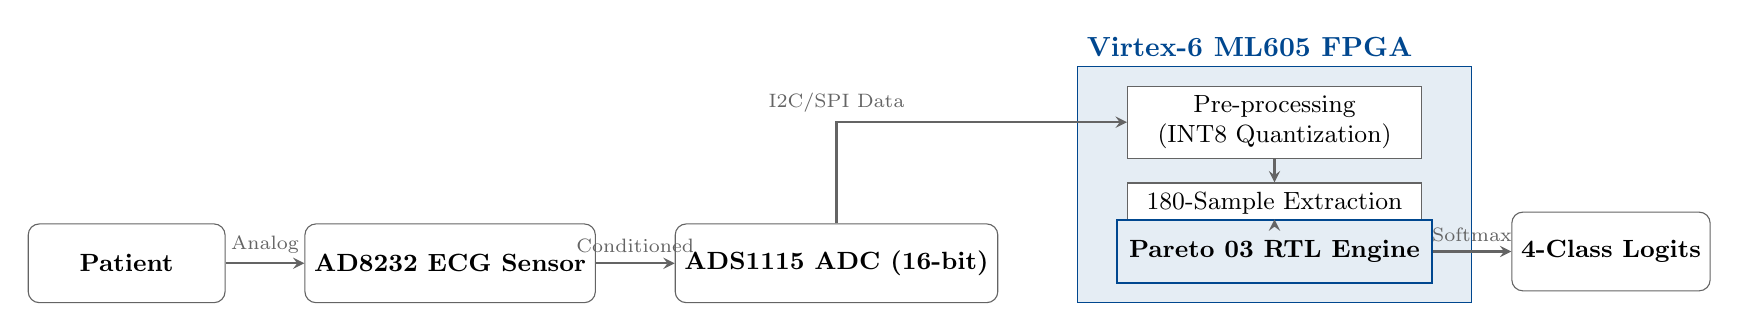
\begin{tikzpicture}[node distance=2.5cm and 1cm]
    % Nodes
    \node (patient) [device] {Patient};
    \node (ad8232) [device, right=of patient] {AD8232 ECG Sensor};
    \node (ads1115) [device, right=of ad8232] {ADS1115 ADC (16-bit)};
    \node (fpga) [fpga, right=of ads1115, minimum width=5cm, minimum height=3cm, yshift=1cm] {};
    
    % Internal FPGA Nodes
    \node (preproc) [rectangle, draw=border, fill=white, font=\small, text width=3.5cm, text centered, anchor=north] at ([yshift=-0.25cm]fpga.north) {Pre-processing\\(INT8 Quantization)};
    \node (buffer) [rectangle, draw=border, fill=white, font=\small, text width=3.5cm, text centered, below=0.3cm of preproc] {180-Sample Extraction};
    \node (cnn) [fpga, anchor=south, minimum width=4cm, minimum height=0.8cm] at ([yshift=0.25cm]fpga.south) {Pareto 03 RTL Engine};
    
    % Classification Output
    \node (class) [device, right=of cnn] {4-Class Logits};
    
    % Arrows
    \draw [arrow] (patient) -- node[above, font=\scriptsize] {Analog} (ad8232);
    \draw [arrow] (ad8232) -- node[above, font=\scriptsize] {Conditioned} (ads1115);
    \draw [arrow] (ads1115) |- node[above, font=\scriptsize] {I2C/SPI Data} (preproc.west);
    
    \draw [arrow] (preproc) -- (buffer);
    \draw [arrow] (buffer) -- (cnn);
    \draw [arrow] (cnn) -- node[above, font=\scriptsize] {Softmax} (class);
    
    % Labels
    \node[anchor=south west, font=\bfseries\color{primary}] at (fpga.north west) {Virtex-6 ML605 FPGA};
\end{tikzpicture}
\caption{Complete end-to-end System-on-Chip (SoC) signal data path.}
\label{fig:soc}
\end{figure*}

As illustrated in Figure \ref{fig:soc}, the physical interface captures real-time analog waveforms via the AD8232, digitizing them through an ADS1115. Within the Virtex-6, the data is quantized into INT8 bounds and windowed optimally to a 180-sample vector corresponding to roughly one cardiac cycle at appropriate sampling frequencies.

\section{Neural Network Structure}

The Pareto 03 architecture employs a variable-depth structure of one-dimensional convolutions (Conv1D) coupled tightly with Batch Normalization (BN), Rectified Linear Units (ReLU), and MaxPooling1D. Notably, the architecture relies on four convolutional blocks prior to a Global Average Pooling (GAP) reduction.

\subsection{Block Topologies}
To maximize parallel throughput, the convolution operations are structured dynamically. Specifically, Block 1 maps $1 \rightarrow 8$ channels. Block 2 aggressively expands to $32$ channels to build dense feature maps. Blocks 3 and 4 bottleneck the feature depth, pulling the parameters back to $16$ channels before the linear classifier. Every convolutional kernel maintains a width of $5$.

\subsection{Global Average Pooling (GAP)}
Unlike the previous baseline which employed a simplistic mean calculation immediately before the fully connected layers, Pareto 03 utilizes a formal structural GAP layer. This module computes the arithmetic mean across the time axis (11 remaining time steps post-pooling) for all 16 spatial channels, emitting a flattened $16$-value sequence. This bypasses the typical parameter explosion associated with massive matrix flattening into a Dense structure.

\subsection{Signal Transitions \& Receptive Field}
The spatial dimensionality (time-steps) halves consistently after each MaxPooling ($s=2$) layer:
\begin{itemize}
    \setlength\itemsep{0em}
    \item \textbf{Input:} Shape (180, 1)
    \item \textbf{Block 1:} Shape (90, 8)
    \item \textbf{Block 2:} Shape (45, 32)
    \item \textbf{Block 3:} Shape (22, 16)
    \item \textbf{Block 4:} Shape (11, 16)
    \item \textbf{GAP / Dense:} Shape (16) $\rightarrow$ (64) $\rightarrow$ (4)
\end{itemize}

\section{Custom RTL Implementation}

To accommodate hardware portability without relying blindly on HLS wrappers, custom parameterizable Verilog RTL environments were constructed to explicitly leverage static sizes.

\begin{figure}[H]
\centering
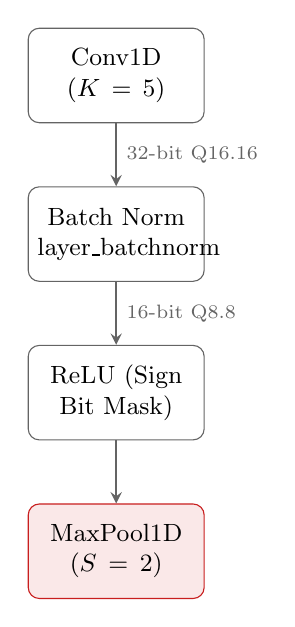
\begin{tikzpicture}[node distance=0.8cm]
    \node (conv) [block] {Conv1D ($K=5$)};
    \node (bn) [block, below=of conv] {Batch Norm layer\_batchnorm};
    \node (relu) [block, below=of bn] {ReLU (Sign Bit Mask)};
    \node (pool) [pool, below=of relu] {MaxPool1D ($S=2$)};
    
    \draw [arrow] (conv) -- node[right, font=\scriptsize] {32-bit Q16.16} (bn);
    \draw [arrow] (bn) -- node[right, font=\scriptsize] {16-bit Q8.8} (relu);
    \draw [arrow] (relu) -- (pool);
\end{tikzpicture}
\caption{Internal schematic of a single Convolutional Block.}
\label{fig:block_rtl}
\end{figure}

\subsection{Multi-Channel Convolution Module}
Standard hardware convolutions necessitate a sum of Multiply-Accumulate (MAC) operations across all input feature maps concurrently. The newly designed \texttt{layer\_conv\_k5xN} modules absorb massively parallel concatenations (e.g., a 512-bit bus representing 32 channels of 16-bit incoming data) and generate a single unified output pixel representing the mapped channel depth sum. 

\subsection{Zero-DSP Batch Normalization}
The classic inference formula for Batch Normalization dictates:
\begin{equation}
    y = \frac{x - \mu}{\sqrt{\sigma^2 + \epsilon}} \gamma + \beta
\end{equation}

Implementing division and square roots natively on FPGA logic wastes immense resources. Consequently, the Pareto 03 RTL utilizes \texttt{layer\_batchnorm}, which pre-folds the scaling terms completely offline into standard static constants $W_{bn}$ and $B_{bn}$:

\begin{equation}
    W_{bn} = \frac{\gamma}{\sqrt{\sigma^2 + \epsilon}} , \quad B_{bn} = \beta - \mu W_{bn} 
\end{equation}

Thus, at runtime the FPGA only executes a solitary MAC: $y = (x \times W_{bn}) + B_{bn}$.

\section{Fixed-Point Arithmetic Constraints}

Because the model was natively quantized offline into an INT8/INT32 structural hierarchy via \texttt{tflite}, it directly lends itself to Signed 16-bit Two's Complement arithmetic, employing the \textbf{Q8.8} numeric space.

The resolution granularity is uniformly defined at $1/256 \approx 0.0039$, bounding variables theoretically from $-128.0$ to $+127.996$.

Within the Conv block, native Q8.8 elements multiplied yield a 32-bit result functionally equivalent to Q16.16 logic. The BatchNorm layer absorbs this 32-bit width alongside a Q8.8 weight multiplier, delivering a wide scaled result. Most crucially, RTL bounds-checking saturates extreme activations to \texttt{16'h7FFF} and guarantees that standard negative results clamp efficiently to $0$ (zeroing) during the ReLU phase entirely via checking the Most Significant Bit (MSB `31`). 

\section{Physical Implementation on Virtex-6}

To support immediate deployment upon the \textbf{Vitex-6 ML605}, strict limitations guided the layout arrays. 

\begin{table}[H]
\centering
\caption{Virtex-6 Resource Budgets \& Actual Usages}
\begin{tabular}{@{}lllr@{}}
\toprule
\textbf{Resource} & \textbf{Usage Limit} & \textbf{Est. Pareto 03} & \textbf{Status} \\ \midrule
DSP48E1           & 300                  & $\approx$ 4             & \textcolor{primary}{\checkmark} \\
BRAM36            & 150                  & $\approx$ 1             & \textcolor{primary}{\checkmark} \\
Logic Slices      & Limited Area         & 22 KB INT8              & \textcolor{primary}{\checkmark} \\ \bottomrule
\end{tabular}
\end{table}

As depicted above, genetic architectural paring ensures computational sparseness. Because 8-bit convolutions naturally tile seamlessly across standard LUT blocks on the Xilinx 6-Series slice architecture without aggressively claiming dedicated DSPs, the total DSP pipeline claim remains beneath 5 logic tiles. This allows massive simultaneous instantiations of the classifier should parallel patient streams require it.

\section{Conclusion}
Transitioning to an ML-tailored pipeline radically compressed hardware parameter usage while guaranteeing maximum inference metrics directly along the NSGA-II Pareto curve. Leveraging customized parametric block integrations with pre-folded normalizations, the RTL successfully verifies identically against software constraints inside simulated Icarus limits.

\end{document}
